\chapter{Desarrollo de APIs}

En este capítulo se hablará sobre las diferentes librerías (APIs) que se han realizado en este proyecto, explicando detalladamente la estructura de cada una de ellas.

Por último, se hará especial énfasis en el plugin de Net2Plan desarrollado, en el cual se han integrado las difrentes APIs mencionadas anteriormente.


\section{J-OSM Client}
\label{sec:osmclient}

Una de las APIs que se ha desarrollado es un cliente REST para interactuar con OSM (ver sección \ref{sec:osm}).

\begin{figure}[!ht]
	\centering
	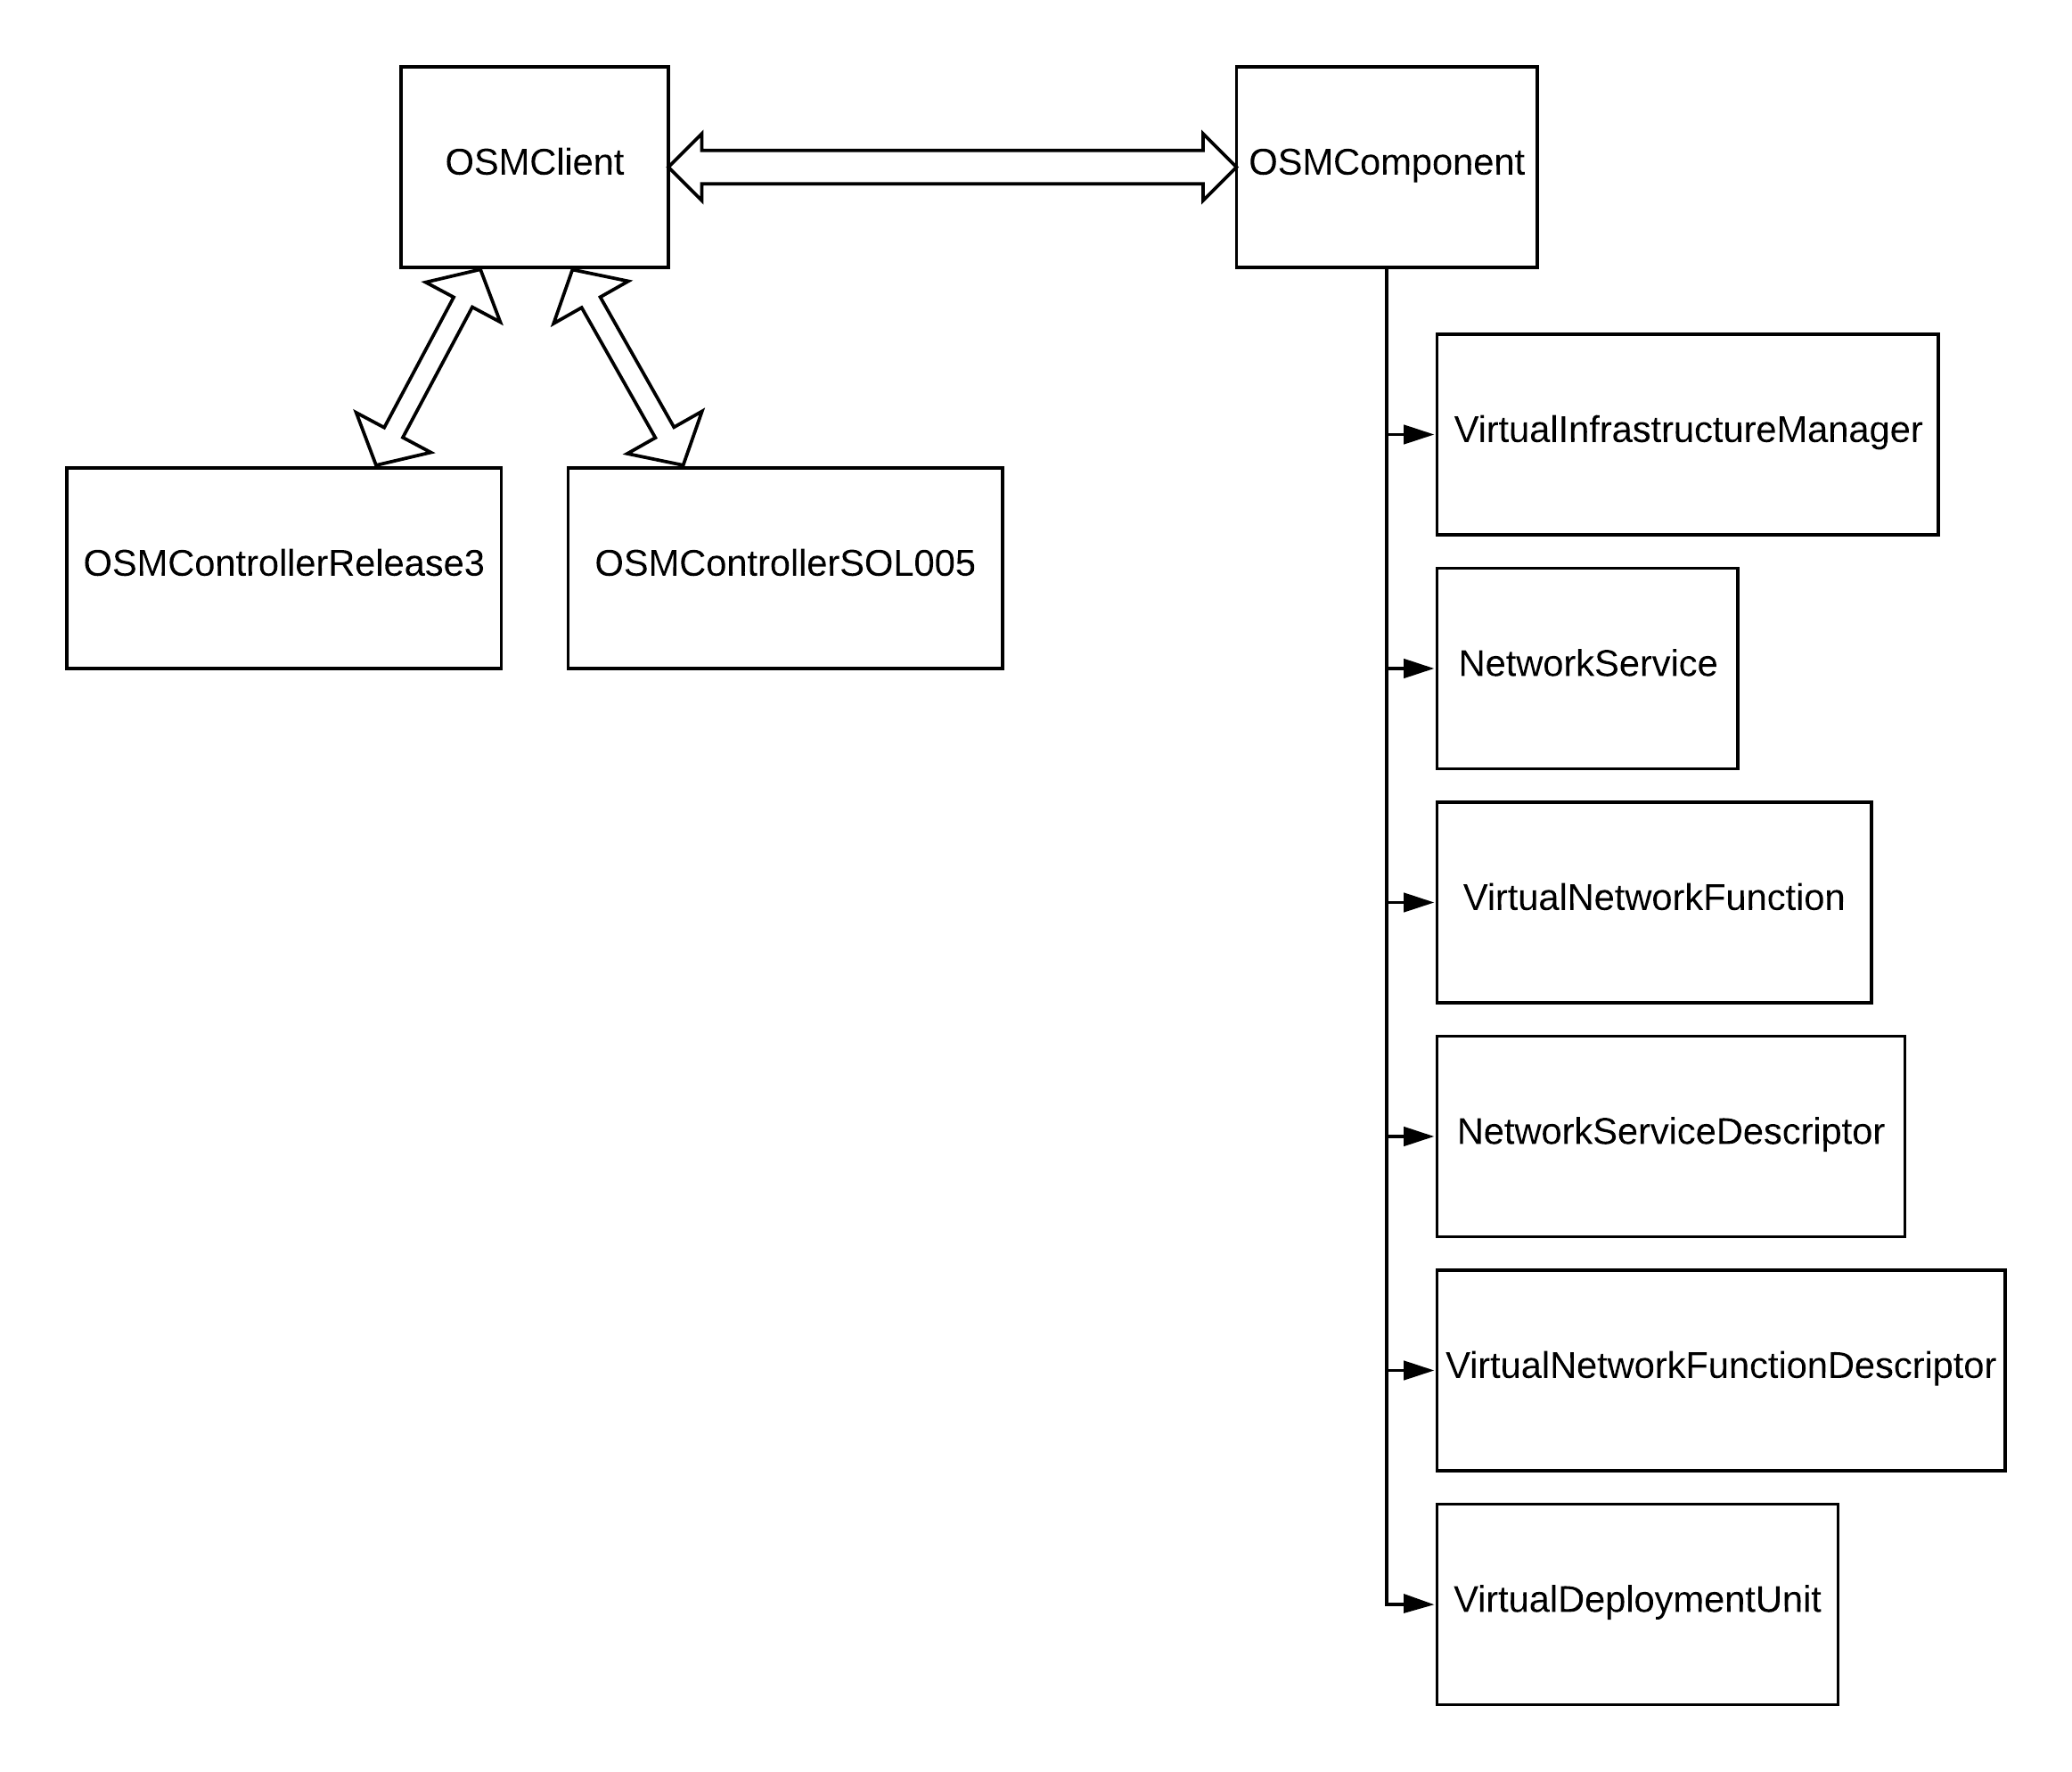
\includegraphics[width=0.7\linewidth]{imagenes/OSMClient}
	\caption{Estructura de clases de J-OSMClient}
	\label{fig:osmclient}
\end{figure}

En la figura \ref{fig:osmclient} se puede ver un esquema detallado de la jerarquía de clases y como dichas clases interaccionan entre sí.


\section{ONOS Client}
\label{sec:onosclient}

\begin{figure}[!ht]
	\centering
	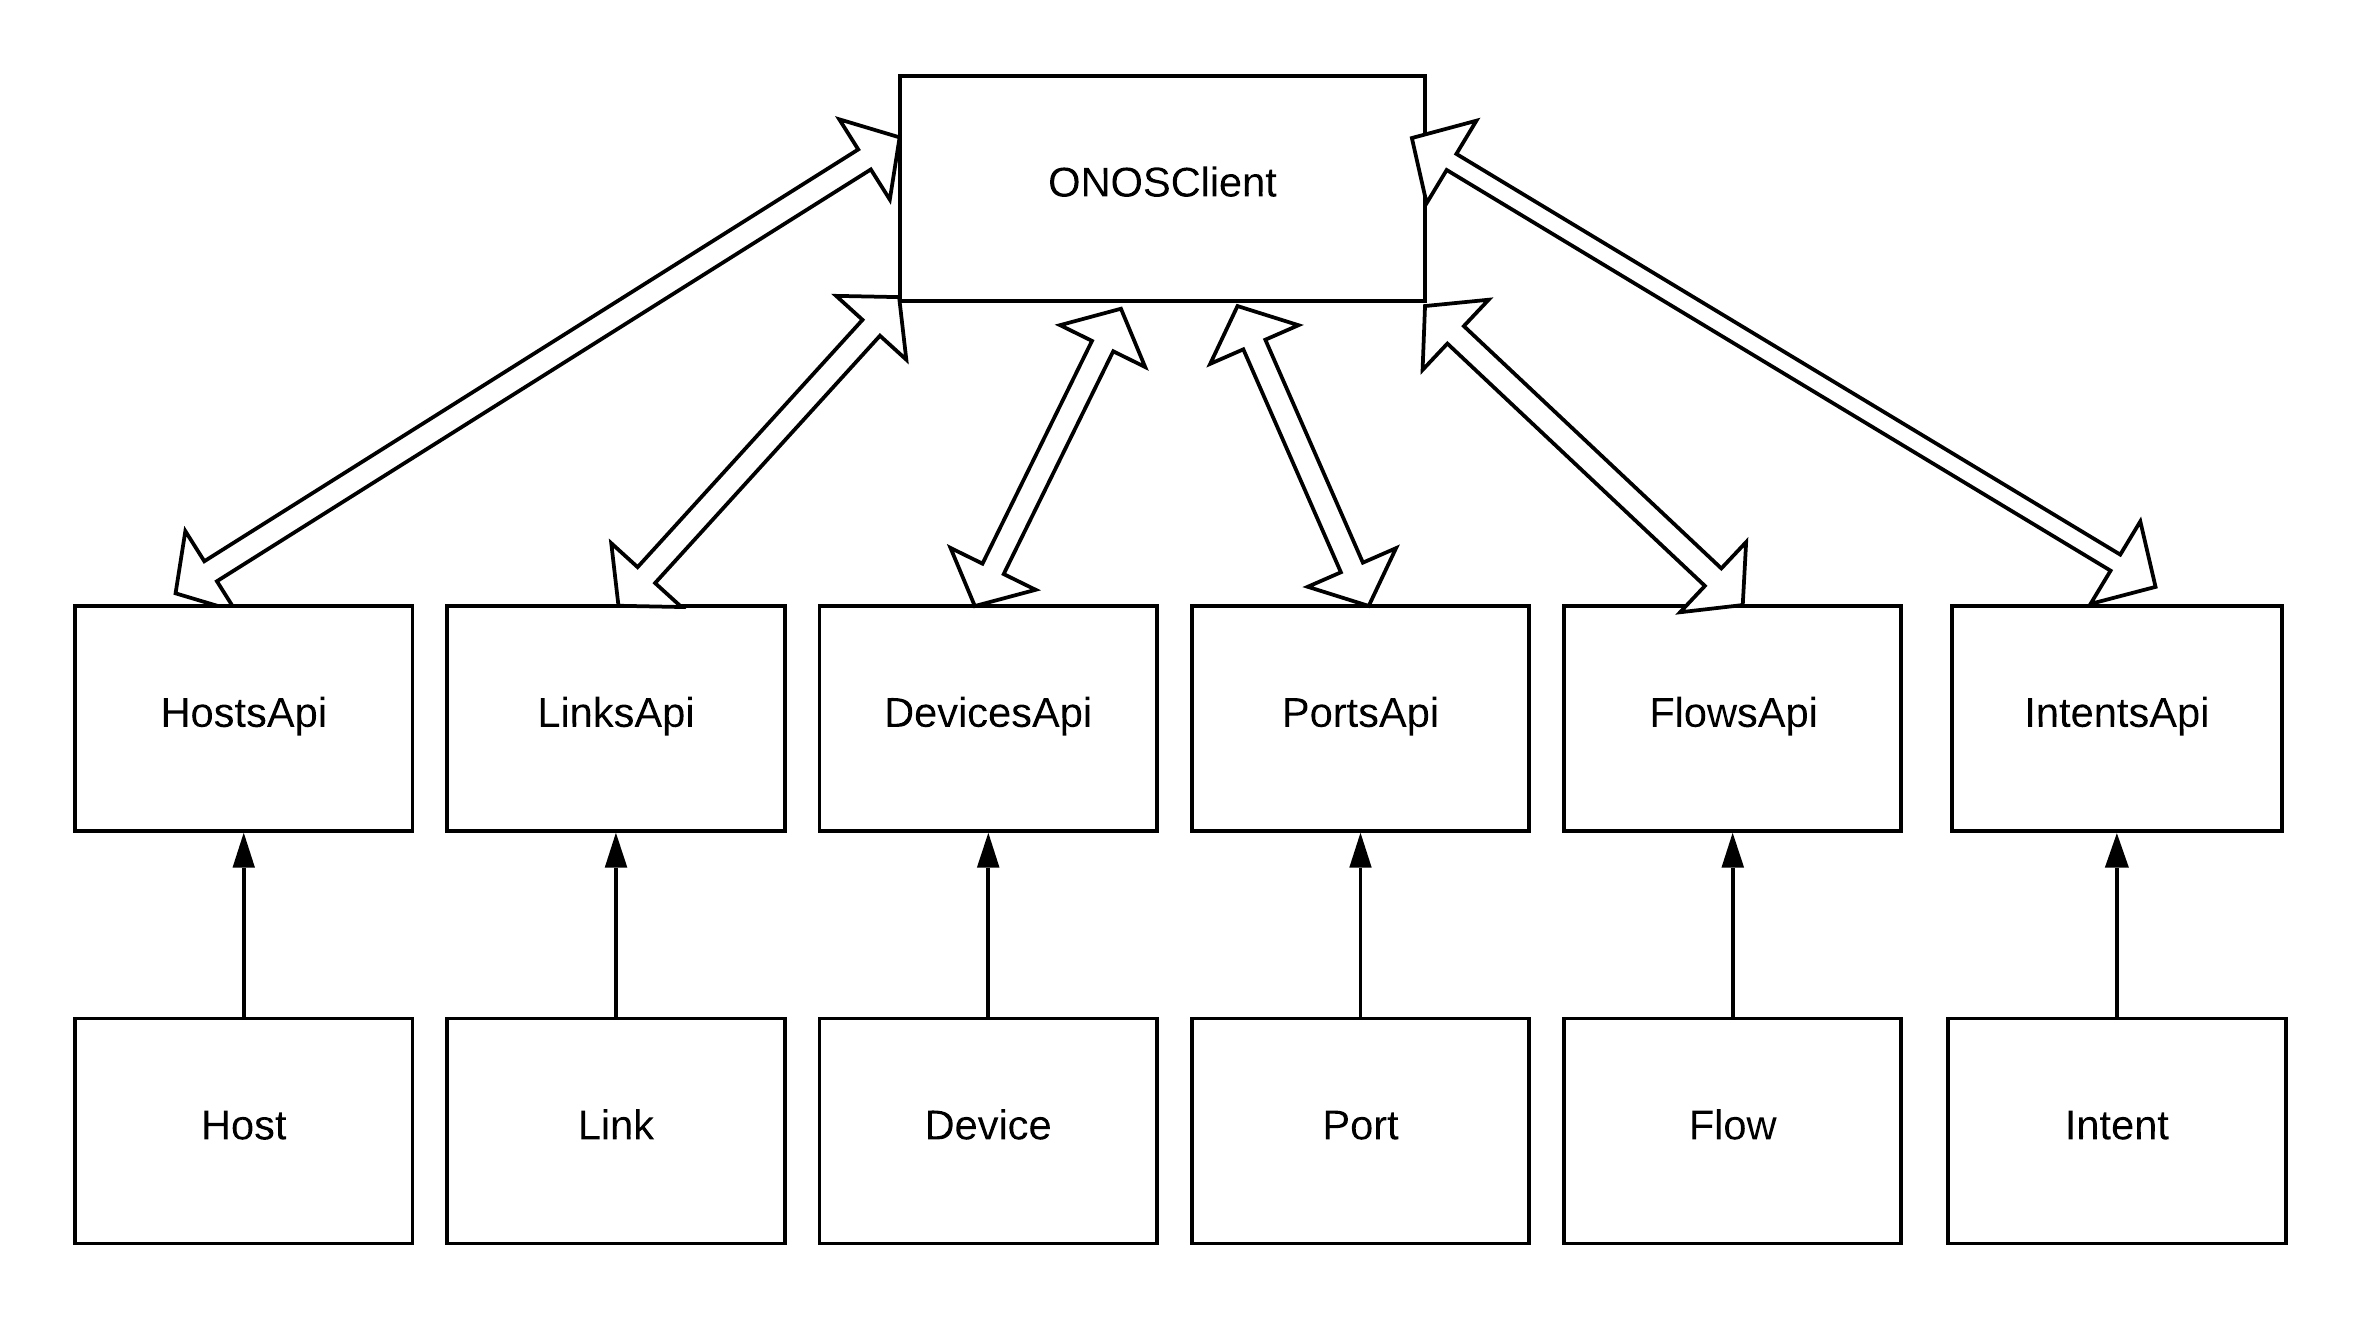
\includegraphics[width=0.7\linewidth]{imagenes/ONOSClient}
	\caption{Estructura de clases de ONOSClient}
	\label{fig:onosclient}
\end{figure}


\section{OpenStack Client}
\label{sec:openstackclient}

\section{Net2Plan: NFV Management Plugin}
\label{sec:nfvplugin}

Para llevar a cabo este proyecto, era necesario integrar las APIs mencionadas anteriormente con una herramienta que tenga funcionalidad de planificación de redes. Por ello, se ha desarrollado una extensión de Net2Plan basada en el plugin Network Design.

\begin{figure}[!ht]
	\centering
	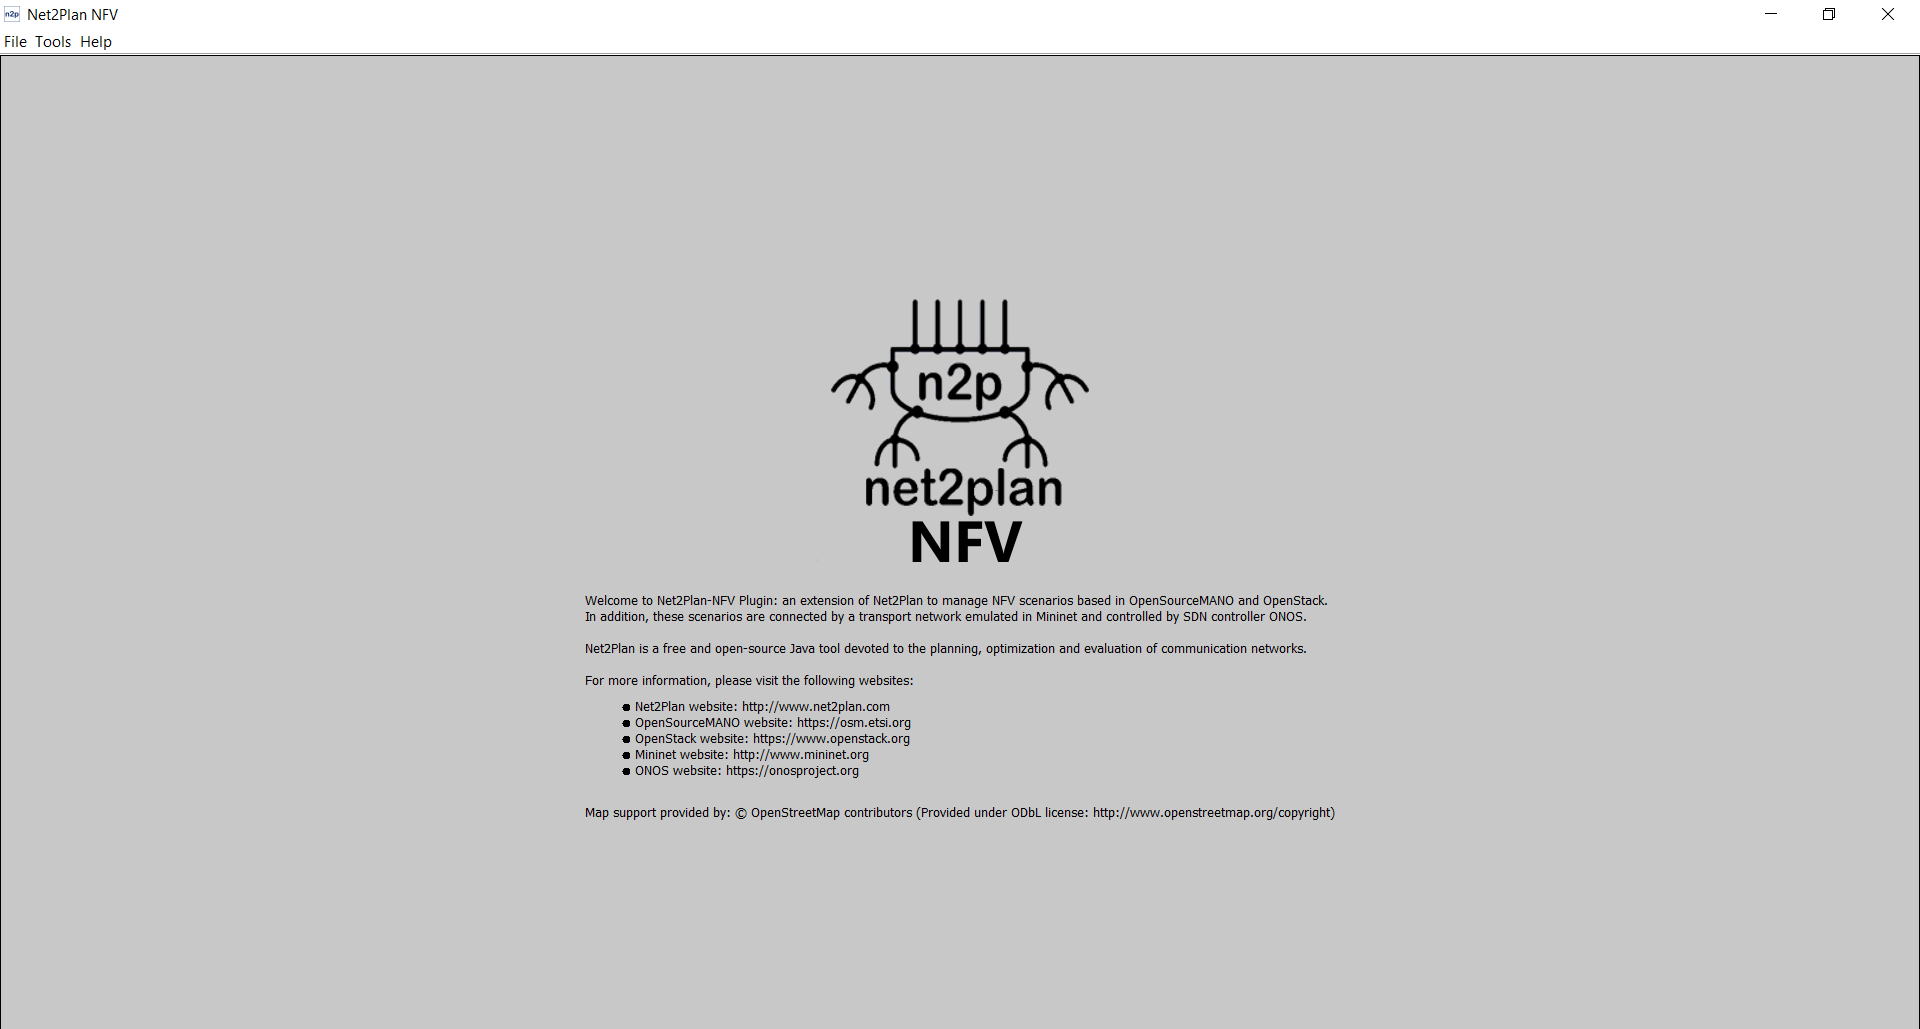
\includegraphics[width=0.8\linewidth]{imagenes/nfvpluginmain}
	\caption{Página de inicio de la extensión Net2Plan-NFV}
	\label{fig:nfvpluginmain}
\end{figure}

\begin{figure}[!ht]
	\centering
	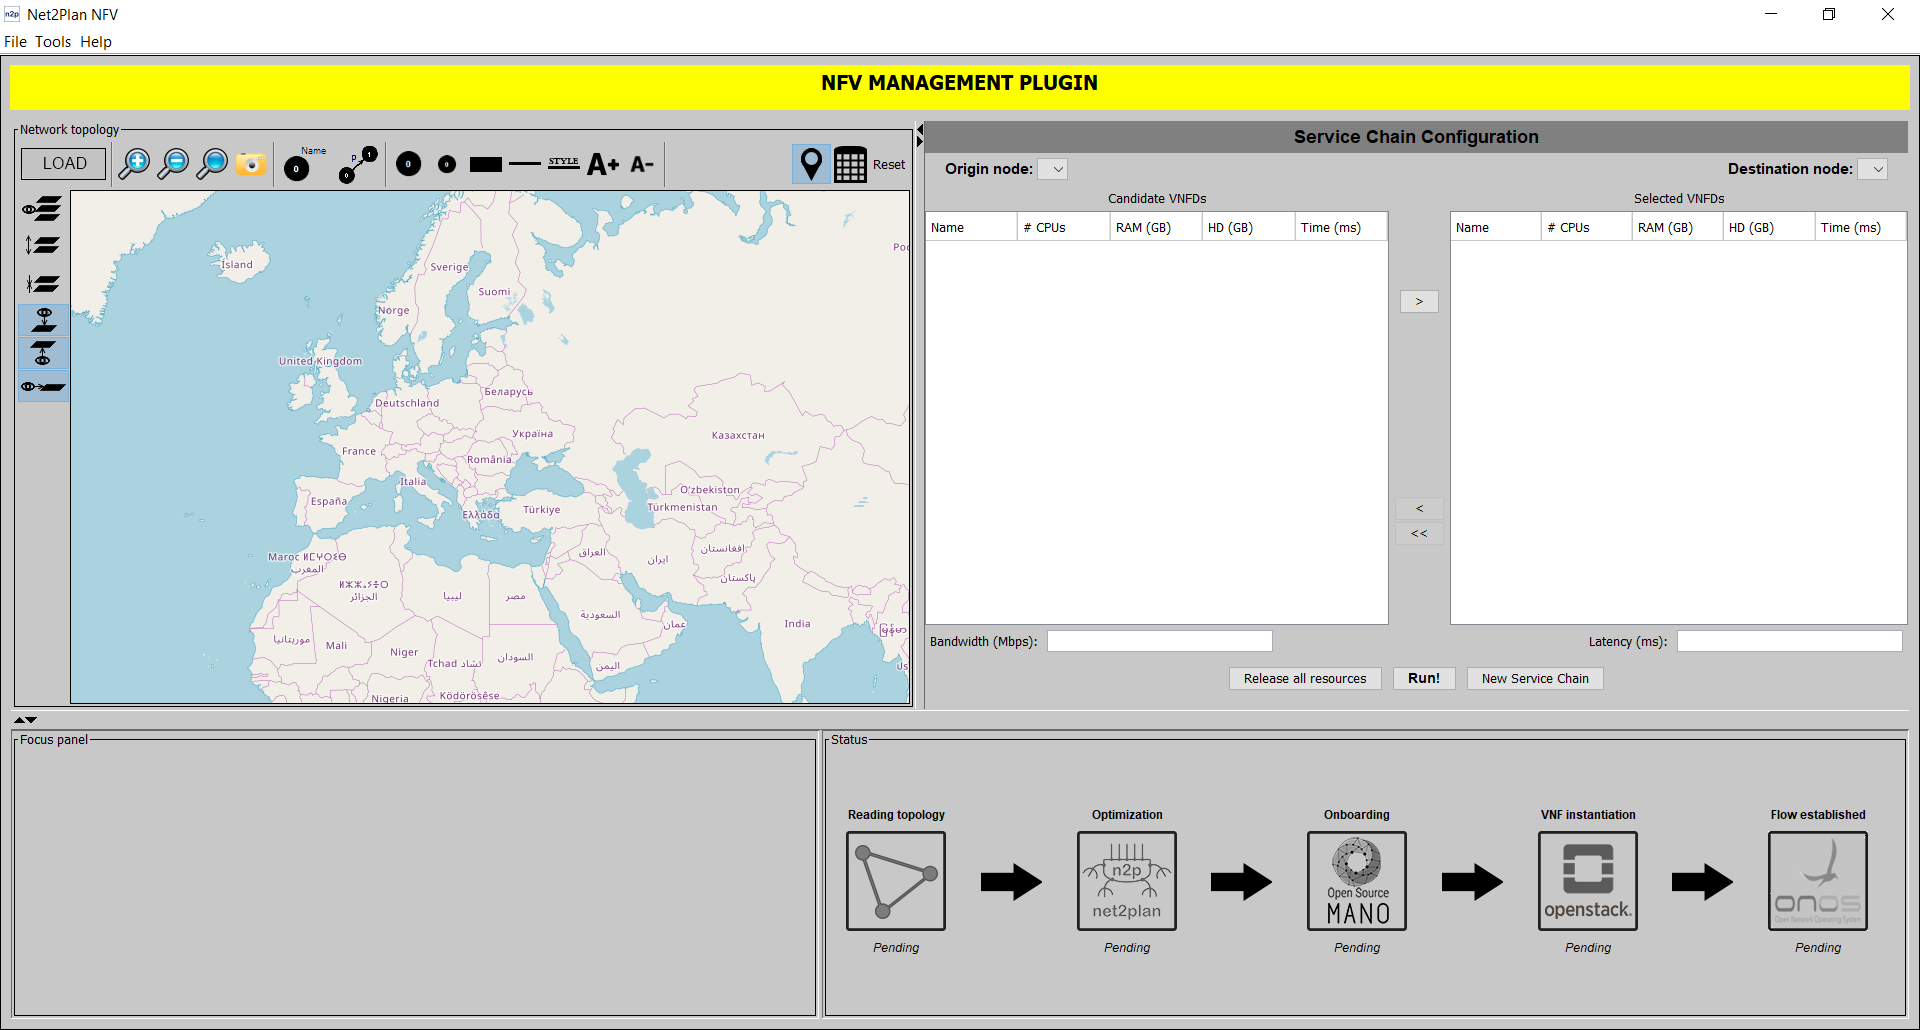
\includegraphics[width=0.8\linewidth]{imagenes/nfvplugin_dashboard}
	\caption{Página de inicio del Plugin NFV-Management}
	\label{fig:nfvplugindash}
\end{figure}






\cleardoublepage